\documentclass[11pt]{standalone}

\usepackage{helvet}

\usepackage{ifthen}
\usepackage{tikz} 
\usetikzlibrary{shapes.misc}
\usetikzlibrary{arrows,arrows.meta}
\usetikzlibrary{calc,intersections, patterns, math}

\definecolor{pfeil}{RGB}{168,167,167}
\definecolor{petrol}{RGB}{0, 118, 136}
\definecolor{darkgoldenrod}{RGB}{184, 134, 11}
\colorlet{petrol-lighter}{petrol!40}
\colorlet{darkgoldenrod-lighter}{darkgoldenrod!40}

\begin{document}

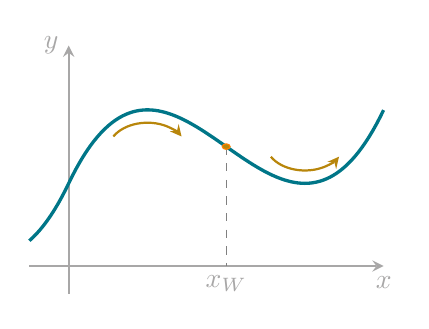
\begin{tikzpicture}[pfeil, yscale=0.7]

    % \draw[thick, fill=petrol!20, draw=petrol-lighter, rounded corners=2ex, opacity=0.5] (0,0) rectangle ++ (1.5,3.5);
    % \draw[thick, fill=darkgoldenrod!20, draw=darkgoldenrod-lighter, rounded corners=2ex, opacity=0.5] (5,0) rectangle ++ (1.5,3.5);

    \draw[thick, -stealth] (-0.5,0) -- (4,0) node[below] {$x$};
    \draw[thick, -stealth] (0,-0.5) -- (0,4) node[left] {$y$};
    \draw[very thick, petrol, domain=-0.5:4, samples = 100] plot(\x,{1/3*\x^3-2*\x^2+3*\x+1.5}) ;
    \draw[dashed, gray] (2,2.1666666) -- (2,0) node[below] {\color{pfeil}$x_W$};
    \draw[orange,fill=darkgoldenrod] (2,2.1666666) circle (0.05);
    
    \draw[-stealth, thick, darkgoldenrod] (1,2.1) ++(150:0.5) arc(150:30:0.5);
    \draw[-stealth, thick, darkgoldenrod] (3,2.233333) ++(210:0.5) arc(210:330:0.5);

\end{tikzpicture}

\end{document}
